\emph{Authors}: Gigi Johnson and Joe Corneli

\begin{quote}
So you've decided you want to try peer learning? Maybe you've already
found a few people who will support you in this effort. Congratulations!
It's time now to focus your thinking. How will you convene others to
form a suitable group? How will you design a learner experience which
will make your project thrive? In this chapter, we suggest a variety of
questions that will help you to make your project more concrete for
potential new members. There are no good or bad answers - it depends on
the nature of your project and the context. Trying to answer the
questions is not something you do just once. At various stages of the
project, even after it's over, some or all of those questions will
aquire new meanings - and probably new answers.
\end{quote}
\begin{quote}
\textbf{Fabrizio Terzi}:
There is a force of attraction that allows aggregation into
groups based on the degree of personal interest; the ability to enhance
and improve the share of each participant; and the expectation of success
and potential benefit.
\end{quote}
\subsection{Group identity}

Note that there are many groups that may not need to be ``convened'',
since they already exist. There is a good story from
\href{http://www.sarvodayausa.org/learn/a-t-ariyartne/}{A. T.
Ariyaratne} in his
\href{http://www.sarvodaya.org/about/philosophy/collected-works-vol-1/rural-self-help}{collected
works} in which he does ``convene'' a natural group (namely, a village)
- but in any case, keep in mind at the outset that the degree of
group-consciousness that is necessary for peer learning to take place is
not fixed. In this section, we suppose you are just at the point of
kicking off a project. What steps should you take? We suggest you take a
moment to ponder the following questions first - and revisit them
afterward, as a way to identify best practices for the next effort.

\subsection{There will be a quiz}

Those taking the initiative should ask themselves the traditional Who,
What, Where, When, Why, and How.
(\href{http://en.wikipedia.org/wiki/Simon\_Sinek}{Simon Sinek} suggests
to begin with Why, and we touched on Who, above!). In doing so,
preliminary assumptions for design and structure are established.
However, in peer learning it is particularly important to maintain a
healthy degree of openness, so that future group members can also form
their answers on those questions. In particular, this suggests that the
design and structure of the project (and the group) may change over
time. Here, we riff on the traditional 5W's+H with six clusters of
questions to help you focus your thinking about the project and amplify
its positive outcomes.

\begin{center}
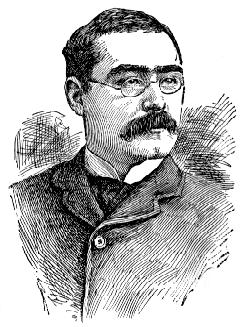
\includegraphics[width=.5\textwidth]{../pictures/kipling.jpg} \\
``I keep six honest serving-men (They taught me all I knew)''
\end{center}

\subsection{Expectations for participants}

\textbf{1. Who: Roles and flux}

\begin{itemize}
\item
  What are some of the roles that people are likely to fall into (e.g.
  Newcomer, Wrapper, Lurker, Aggregator, etc.)?
\item
  How likely is it that participants will stick with the project? If you
  expect many participants to leave, how will this effect the group and
  the outcome?
\item
  Do you envision new people joining the group as time goes by? If so,
  what features are you designing that will support their integration
  into an existing flow?
\item
  Will the project work if people dip in and out? If so, what features
  support that? If not, how will people stay focused?
\end{itemize}
\textbf{2. What: Nature of the project}

\begin{itemize}
\item
  What skills are required? What skills are you trying to build?
\item
  What kinds of change will participants undergo? Will they be heading
  into new ground? Changing their minds about something? Learning about
  learning?
\item
  What social objective, or ``product'' if any, is the project aiming to
  achieve?
\item
  What's the `hook?' Unless you are working with an existing group, or
  re-using an existing modality, consistent participation may not be a
  given.
\end{itemize}
\textbf{3. When: Time management}

\begin{itemize}
\item
  What do you expect the group to do, from the moment it convenes, to
  the end of its life-span, to create the specific outcome that will
  exist at the conclusion of its last meeting? (C. Gersick.) Note that
  what people ACTUALLY do may be different from what you envision at the
  outset, so you may want to revisit this question (and your answer)
  again as the project progresses.
\item
  Keeping in mind that at least one period of is inertia is very likely
  (C. Gersick), what event(s) do you anticipate happening in the group
  that will bring things back together, set a new direction, or
  generally get things on track? More generally, what kinds of
  contingencies does your group face? How does it interface to the
  ``outside world''?
\item
  What pre-existing narratives or workflows could you copy in your
  group?
\item
  How much of a time commitment do you expect from participants? Is this
  kind of commitment realistic for members of your group?
\item
  What, if anything, can you do to make participation ``easy'' in the
  sense that it happens in the natural flow of life for group members?
\item
  Does everyone need to participate equally? How might non-equal
  participation play out for participants down the line?
\end{itemize}
\textbf{4. Where: Journey vs Destination}

\begin{itemize}
\item
  What structures will support participants in their journey to the end
  result(s) you (or they) have envisioned? What content can you use to
  flesh out this structure?
\item
  Where can the structure ``flex'' to accommodate unknown developments
  or needs as participants learn, discover, and progress?
\end{itemize}
\textbf{5. Why: Tool/platform choice}

\begin{itemize}
\item
  What tools are particularly suited to this group? Consider such
  features as learning styles and experiences, geographical diversity,
  the need for centralization (or de-centralization), cultural
  expectations related to group work, sharing, and emerging leadership.
\item
  Is there an inherent draw to this project for a given population, or
  are you as facilitator going to have to work at keeping people
  involved? How might your answer influence your choice of tools? Is the
  reward for completion the learning itself, or something more tangible?
\item
  In choosing tools, how do you prioritize such values and objectives as
  easy entry, diverse uses, and high ceilings for sophisticated
  expansion?
\end{itemize}
\textbf{6. How: Linearity vs Messiness}

\begin{itemize}
\item
  How will your group manage feedback in a constructive way?
\item
  Why might participants feel motivated to give feedback?
\item
  How firm and extensive are the social contracts for this group? Do
  they apply to everyone equally, or do they vary with participation
  level?
\item
  What do people need to know at the start? What can you work out as you
  go along? Who decides?
\item
  How welcome are ``meta-discussions''? What kinds of discussions are
  not likely to be welcome? Do you have facilities in place for
  ``breakout groups'' or other peer-to-peer interactions?
  (Alternatively, if the project is mostly distributed, do you have any
  facilities in place for coming together as a group?)
\end{itemize}
\subsection{Cycles of group development}

The above questions remain important thoughout the life of the project.
People may come and go, particpants may propose fundamentally new
approaches, people may evolve from lurkers to major content creators or
vice-versa. The questions we suggest can be most effective if your group
discusses them over time, as part of its workflow, using synchronous
online meetings (e.g., Big Blue Button, Adobe Connect, Blackboard Collaborate), forums, Google docs, wikis, and/or email lists. Regular
meetings are one way to establish a ``heartbeat'' for the group.

In thinking about other ways of structuring things, note that the
``body'' of the \emph{Peeragogy Handbook} follows a
\href{http://en.wikipedia.org/wiki/Forming-storming-norming-performing}{Tuckman-like
outline} (\emph{Convening a Group} is our ``forming'', \emph{Organizing
a Learning Context} is our ``storming and norming'',
\emph{Co-working/Facilitation} is our ``performing'', and
\emph{Assessment} is our ``adjourning''). But we agree with Gersick
{[}1{]}, and Engeström {[}2{]}, that groups do not always follow a
linear or cyclical pattern with their activities!

Nevertheless, there may be some specific stages or phases that you want
\emph{your} group to go through. Do you need some ``milestones,'' for
example? How will you know when you've achieved ``success?''

%\subsection{Dealing with chaos or conflict}

In closing, it is worth reminding you that it is natural for groups to
experience conflict, especially as they grow or cross other threshold
points or milestones - or perhaps more likely, when they don't cross
important milestones in a timely fashion (ah, so you remember those
milestones from the previous section!). Nevertheless, there are some
strategies can be used to make this conflict productive, rather than
merely destructive (see Ozturk and Simsek {[}3{]}).

\subsection{References}

\begin{enumerate}
\item
  Engeström, Y. (1999). Innovative learning in work teams: Analyzing
  cycles of knowledge creation in practice. In Y. Engeström, R.
  Miettinen \& R.-L-. Punamäki (Eds.), \emph{Perspectives on activity
  theory}, (pp. 377-404). Cambridge, UK: Cambridge University Press
\item
  Gersick, C. (1988). Time and transition in work teams: Toward a new
  model of group development. \emph{Academy of Management Journal} 31
  (Oct.): 9-41.
\item
  Ozturk and Simsek, ``\href{http://networkedlearningconference.org.uk/abstracts/pdf/ozturk.pdf}{Of Conflict in Virtual Learning Communiities in
  the Context of a Democratic Pedagogy: A paradox or sophism?},'' in
  \emph{Proceedings of the Networked Learning Conference, 2012,
  Maastricht.} 
\end{enumerate}
